\section{Basic Concepts of Federated Learning}

\subsection{Definition}
Federated Learning~\cite{IEEEstd3652, mcmahan2017communication} is a collaborative machine learning modeling paradigm that enables sharing and aggregation of knowledge from multiple sources while maintaining the confidentiality of source data.
Generally, in terms of task organization, there are two kinds of entities in FL systems: the server and participant. 
The FL server can launche a federated training task and invites participants with sufficient training data and hardware resources to contribute their local modeling results for multi-source knowledge aggregation.
In practice, FL systems can be divided into two categories based on application scenarios~\cite{kairouz2021advances}:
\begin{itemize}
    \item Cross-device FL. In this setting, the participants are numberous end devices with relatively small dataset size, such as mobiles, IoT sensors and wearable devices, the server is hosted in the cloud. Since there is low context correlation between the data of distributed end devices and less overlapping sample ids, this setting typically falls within the scope of horizontal FL. The cross-device FL applications include: Gboard next-word prediction~\cite{hard2018federated}, emoji prediction~\cite{ramaswamy2019federated} and query suggesion~\cite{yang2018applied}.
    \item Cross-silo FL. In this setting, the participants are orginizations or institutions with large amounts of well-maintained structured data, and the server is hosted by a trusted FL service providers such as FATE~\cite{liu2021fate} and NVFLARE~\cite{roth2022nvidia}. As participants can be different departments within an organization, the data silo owned by these departments can have a large overlap in sample space and less overlap in feature space, which falls within vertical FL. The applications of cross-silo FL include federated data analysis for radiomics~\cite{li2019privacy, li2020multi, scherer2020joint}, epidemiology~\cite{dayan2021federated} and EHR~\cite{brisimi2018federated, huang2019patient}.
\end{itemize}

The allocation to the server and participants in FL is dependent on the particular application context. 
Furthermore, FL entities can also serve multiple functional roles to support advanced features such as privacy enhancement~\cite{geyer2017differentially, bonawitz2017practical}, participant scheduling~\cite{li2022federated, abdulrahman2020fedmccs}, model verification~\cite{tekgul2021waffle, shao2022fedtracker} and incentive mechanisms~\cite{yu2020fairness}.
Recall that there are four roles defined in the FL standard~\cite{IEEEstd3652}:

\begin{itemize}
    \item Model User. The FL model users can request for FL modeling services and preset the targeted task, and then establish cooperation with participants who provide training data. This role can leverage the benefits of collaborative training to improve the preformance of its objective models.
    \item Coordinator. The FL coordinator is responsible for providing FL services to all FL entities. This role involves setting up communication channels with entities, initializing the execution environment~\cite{hanzlik2021mlcapsule} of participants, scheduling the training and aggregation workflows for improve system efficiency, such as by alleviating the straggler effect~\cite{li2021fedsae, chai2020tifl}, optimizing data heterogeneity~\cite{duan2019astraea, abdulrahman2020fedmccs} and compressing model transfer~\cite{konevcny2016federated, sattler2019robust}.
    Additionaly, the FL coordinator provides privacy control mechanisms~\cite{bonawitz2017practical, el2022differential, hesamifard2018privacy} for model users and authorization verification for participants to maintain the security of FL systems. 
    Furthermore, the coordinator can hold a validation dataset for evaluate the models contributed by participants or detect potential disturbances from Byzantine attacks~\cite{sattler2020byzantine}.
    \item Data Owner. The FL data owners
    \item Auditor
\end{itemize}


\begin{figure}[t]
    \centering
    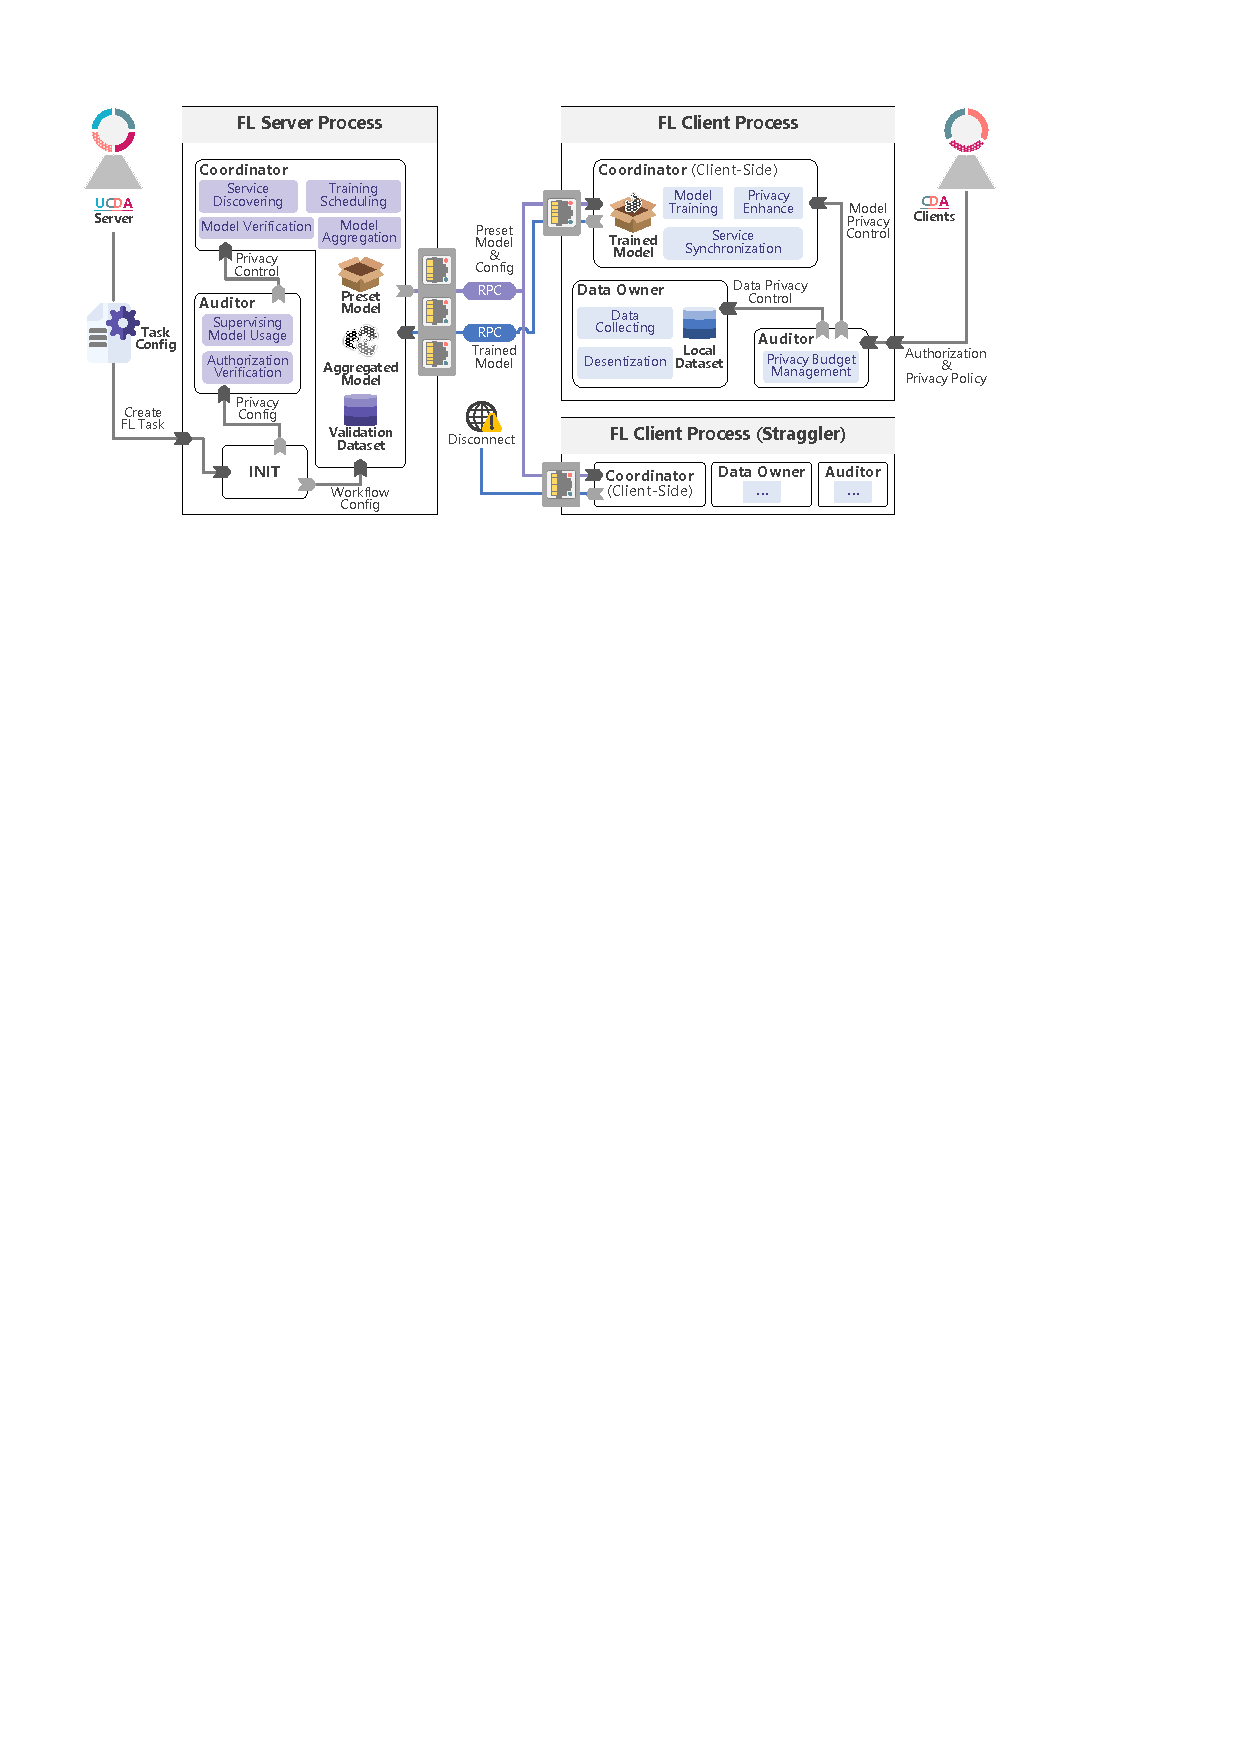
\includegraphics[width=\linewidth]{fig/fl_frame.pdf}
    \caption{An overview of traditional FL systems. (U: model User, C: Coordinator, D: Data owner, A: Auditor)}
    \Description{}
    \label{fig:fl}
  \end{figure}